\documentclass[11pt]{article}
\usepackage{amsmath, amscd, amssymb, amsthm}
% \usepackage{diagrams}
\usepackage{color}
\usepackage{graphicx, psfrag, tikz}
\usepackage[all]{xy}
\usepackage[margin=1in]{geometry}

\usepackage{enumitem,kantlipsum}
\usetikzlibrary{arrows.meta}
\usetikzlibrary{calc,patterns,angles,quotes}
%\renewcommand{\baselinestretch}{1.17}
\usepackage{chemformula}

\newtheorem{theorem}{Theorem}[section]
\newtheorem{lemma}[theorem]{Lemma} 
\newtheorem{proposition}[theorem]{Proposition}
\newtheorem{corollary}[theorem]{Corollary}
\theoremstyle{definition} 
\newtheorem{definition}[theorem]{Definition}
\newtheorem{conjecture}[theorem]{Conjecture}
\newtheorem{remark}[theorem]{Remark}
\newtheorem{example}[theorem]{Example}


\begin{document}
\begin{center}
\textbf{Math 309 Homework 7}\\
(6 problems)
\end{center}



\begin{enumerate}[leftmargin=*]
\item 
Consider the system of 2nd order equations
$$
\begin{cases}
x''=ny\\
y''=-nx
\end{cases},
$$
where $n\geq 1$ is some constant.  Now we write this as an equivalent system of 1st order equations
$$
\begin{cases}
x_1'=x_2\\
x_2'=ny_1\\
y_1'=y_2\\
y_2'=-nx_1
\end{cases}, \quad \text{i.e. } 
\begin{bmatrix}x_1' \\ x_2' \\y_1'\\y_2' \end{bmatrix} 
= A\begin{bmatrix}x_1\\x_2\\y_1\\y_2\end{bmatrix}, \quad \text{where } 
A=\begin{bmatrix}0 &1&0&0\\
0&0&n&0\\
0&0&0&1\\
-n&0&0&0
\end{bmatrix}.
$$
Find the general solution to the above system of first order equations in terms of real valued functions.\\

\textbf{Hint:} here I explain and provide the eigenvalues and eigenvectors of the matrix $A$.   Then you can just use the eigenvalues and eigenvectors that I boxed below without explanation.  To find the eigenvalues, we need to find $\lambda$ such that 
\begin{eqnarray*}
& & \det(A-\lambda I)= \lambda^4+n^2=0\\
&\Rightarrow & \lambda^4=-n^2\\
& \Rightarrow & \lambda=(-1)^{\frac{1}{4}}\sqrt n.
\end{eqnarray*}
Note that $-1=e^{i k\pi}=\cos(k\pi)+i\sin(k\pi)$, where $k$ is an odd integer.  So the 4th roots of $-1$ are 
\[
(-1)^{\frac{1}{4}}=e^{\frac{i k\pi}{4}}=\cos\frac{k\pi}{4}+i\sin\frac{k\pi}{4}.
\]
From this it appears like there are infinitely many 4th roots of $-1$, one for each odd integer $k$; however, most of these are repetitions since cosine and sine are $2\pi$ periodic.  Distinct roots can be represented by the $k$'s where $\frac{k\pi}{4}$ are in a $2\pi$ interval such as  $(-\pi, \pi]$, which are $k=\pm 1, \pm 3$ that correspond to $\frac{k\pi}{4}=\pm \frac{\pi}{4}, \pm \frac{3\pi}{4}$.  So there are four 4th roots of $-1$, which are given by
\begin{eqnarray*}
& & e^{\frac{\pi i}{4}}=\cos \frac{\pi}{4}+i \sin \frac{\pi}{4}=\frac{1}{\sqrt 2}+i\frac{1}{\sqrt 2},\\
& &e^{-\frac{\pi i}{4}}=\cos\left(- \frac{\pi}{4}\right)+i \sin\left(- \frac{\pi}{4}\right)=\frac{1}{\sqrt 2}-i\frac{1}{\sqrt 2},\\
& & e^{\frac{3\pi i}{4}}=\cos \frac{3\pi}{4}+i \sin \frac{3\pi}{4}=-\frac{1}{\sqrt 2}+i\frac{1}{\sqrt 2},\\
&  & e^{-\frac{3 \pi i}{4}}=\cos\left(- \frac{3 \pi}{4}\right)+i \sin\left(- \frac{3\pi}{4}\right)=-\frac{1}{\sqrt 2}-i\frac{1}{\sqrt 2}.
\end{eqnarray*}
Below is a plot of these 4 points on the complex plane
\begin{center}
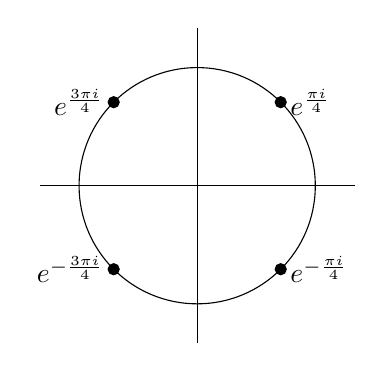
\begin{tikzpicture}
  \draw (0, 0) circle (1.5cm);
 \draw (-2,0) -- (2,0);
 \draw (0, -2)--(0,2);

 \filldraw[black] (1.06066,1.06066) circle (2pt) node[anchor=west] {$e^{\frac{\pi i}{4}}$};     
 \filldraw[black] (1.06066,-1.06066) circle (2pt) node[anchor=west] {$e^{-\frac{\pi i}{4}}$};     
 \filldraw[black] (-1.06066,-1.06066) circle (2pt) node[anchor=east] {$e^{-\frac{3 \pi i}{4}}$};     
 \filldraw[black] (-1.06066,1.06066) circle (2pt) node[anchor=east] {$e^{\frac{3 \pi i}{4}}$};     

\end{tikzpicture}
\end{center}
In summary, the eigenvalues of $A$ are 
\[
\boxed{\sqrt\frac{n}{2}\pm i\sqrt\frac{n}{2}\quad \text{ and} \quad -\sqrt\frac{n}{2}\pm i\sqrt\frac{n}{2}}
\]
 and notice that they come in conjugate pairs which is a consequence of $A$ being a real matrix.  \\

For the conjugate pair $\sqrt \frac{n}{ 2}\pm i\sqrt \frac{n}{2}$, we can find eigenvectors $v$ corresponding to $\sqrt \frac{n}{ 2}+ i\sqrt \frac{n}{2}$ by solving 
\begin{eqnarray*}
\left[A-\left(\sqrt\frac{n}{2}+ i\sqrt\frac{n}{2}\right)I\right]v=
\begin{bmatrix}
-\sqrt\frac{n}{2}- i\sqrt\frac{n}{2}&1&0&0\\
0 &-\sqrt\frac{n}{2}- i\sqrt\frac{n}{2}&n&0\\
0&0& -\sqrt\frac{n}{2}- i\sqrt\frac{n}{2}&1\\
-n&0&0&-\sqrt\frac{n}{2}- i\sqrt\frac{n}{2}
\end{bmatrix}\begin{bmatrix}v_1\\v_2\\v_3\\v_4 \end{bmatrix}=0,
\end{eqnarray*}
i.e.
\begin{eqnarray*}
\text{ \textcircled{1}}& \left(-\sqrt\frac{n}{2}- i\sqrt\frac{n}{2}\right)v_1+v_2=0 \quad & 
\Rightarrow  \quad  v_2= \left(\sqrt\frac{n}{2}+ i\sqrt\frac{n}{2}\right)v_1,   \\
\text{\textcircled{2}}& \left(-\sqrt\frac{n}{2}- i\sqrt\frac{n}{2}\right)v_2+nv_3=0  \quad & \Rightarrow  \quad  v_3=\frac{1}{n}\left(\sqrt\frac{n}{2}+ i\sqrt\frac{n}{2}\right)v_2,   \\
\text{\textcircled{3}} &  \left(-\sqrt\frac{n}{2}- i\sqrt\frac{n}{2}\right)v_3+v_4=0  \quad & \Rightarrow  \quad   v_4=\left(\sqrt\frac{n}{2}+ i\sqrt\frac{n}{2}\right)v_3,  \\
\text{\textcircled{4}}&  -nv_1+\left(-\sqrt\frac{n}{2}- i\sqrt\frac{n}{2}\right)v_4=0 \quad  &\Rightarrow  \quad   v_1=-\frac{1}{n}\left(\sqrt\frac{n}{2}+ i\sqrt\frac{n}{2}\right)v_4.  \\
\end{eqnarray*}
We can take advantage of the fact that $\frac{1}{\sqrt 2}+ i\frac{1}{\sqrt 2}=e^{\frac{i\pi}{4}}$ to make multiplication easier, e.g.  $\left(\frac{1}{\sqrt 2}+ i\frac{1}{\sqrt 2}\right)^2=\left(e^{\frac{i\pi}{4}}\right)^2=e^{\frac{i\pi}{2}}=i$.  We then get that 
\begin{eqnarray*}
\text{\textcircled{2}}\Rightarrow & \quad& v_3= \frac{1}{\sqrt n} e^{\frac{i\pi}{4}}v_2= e^{\frac{i\pi}{2}}v_1=iv_1,\\
\text{\textcircled{3}}\Rightarrow & \quad& v_4= \left(\sqrt\frac{n}{2}+ i\sqrt\frac{n}{2}\right)v_3=i \left(\sqrt\frac{n}{2}+ i\sqrt\frac{n}{2}\right)v_1=\left(-\sqrt\frac{n}{2} + i\sqrt\frac{n}{2}\right)v_1
\end{eqnarray*}
So 
\[
v= \begin{bmatrix}v_1\\v_2\\v_3\\v_4\end{bmatrix}= 
\begin{bmatrix} 1\\ \sqrt \frac{n}{ 2}+ i\sqrt \frac{n}{2}\\ i \\ -\sqrt \frac{n}{ 2}+ i\sqrt \frac{n}{2}\end{bmatrix}v_1, \quad v_1\neq 0 \text{ arbitrary}.
\]
So 
\[
\boxed{\text{an eigenvector corresponding to }\sqrt \frac{n}{ 2}+ i\sqrt \frac{n}{2} \text{ is }\begin{bmatrix} 1\\ \sqrt \frac{n}{ 2}+ i\sqrt \frac{n}{2}\\ i \\ -\sqrt \frac{n}{ 2}+ i\sqrt \frac{n}{2}
\end{bmatrix}}.
\]
For the conjugate pair $-\sqrt \frac{n}{ 2}\pm i\sqrt \frac{n}{2}$, we can find the eigenvectors corresponding to $-\sqrt \frac{n}{ 2}+ i\sqrt \frac{n}{2}$ via a similar calculation and get that 
\[
\boxed{\text{an eigenvector corresponding to }-\sqrt \frac{n}{ 2}+ i\sqrt \frac{n}{2} \text{ is }\begin{bmatrix} 1\\ -\sqrt \frac{n}{ 2}+ i\sqrt \frac{n}{2}\\- i \\ \sqrt \frac{n}{ 2}+ i\sqrt \frac{n}{2}
\end{bmatrix}}.
\]\\


\item Let $f(x)=1$ with $0\leq x\leq \pi$.
\begin{itemize} 
\item[(a)]  Find the Fourier cosine series for $f(x)$.
\item[(b)]   Find the Fourier sine series for $f(x)$.  \\
\end{itemize}

\item
\begin{itemize}
\item[(a)] Solve the given boundary value problem or else show that it has no solution
\[ y''+y=0, \ \ y(0)=0, \ \ y'(\pi)=1.\]

\item[(b)] Solve the given boundary value problem or else show that it has no solution
\[ y''+y=0, \ \ y'(0)=1, \ \ y(L)=0.\]\\
\end{itemize}

\item Find the eigenvalues and eigenfunctions of the given boundary value problem.  
\[y''+\lambda y=0, \ \ y(0)=0, \ \ y'(\pi)=0.\]\\



\item 
\begin{itemize}
\item[(a)] Determine whether the method of separation of variables can be used to replace the given partial differential equation by a pair of ordinary differential equations.  If so, find the equations.  
\[u_{xx}+(x+y)u_{yy}=0.\]

\item[(b)] Determine whether the method of separation of variables can be used to replace the given partial differential equation by a pair of ordinary differential equations.  If so, find the equations.  
\[u_{xx}+u_{yy}+xu=0.\]
\end{itemize}

\item Given a Hamiltonian function $H(x, p)$, the Hamilton-Jacobi equation is 
\[
\frac{\partial W(x, t)}{\partial t}=-H\left(x, \frac{\partial W(x, t)}{\partial x}\right). 
\] 
So for $H(x, p) = \frac{p^2}{2}+V(x)$,  the Hamilton-Jacobi equation for  $W(x, t)$ is 
\[
 \frac{\partial W}{\partial t}=-\frac{1}{2}\left(\frac{\partial W}{\partial x}\right)^2-V(x).\]
\begin{itemize}
\item[(a)] Determine whether the method of separation of variables can be used to replace the above Hamilton-Jacobi equation for $W(x,t)=f(x)g(t)$  by a pair of ordinary differential equations, one for $f(x)$ and one for $g(t)$.  
If so, find the equations.

\item[(b)] Now let us look for solutions of the form $W(x,t)=h(x)+r(t)$.  Find $r(t)$. 
\end{itemize}


\end{enumerate}



\end{document}
